\chapter{Conclusiones}
\label{ch:conclusiones}

En este trabajo se han presentado dos metodologías ágiles que junto
con la expuesta por Dña. Simona se han extraído una serie de
características comunes y comparado con otras metodologías más
tradicionales. En el Cuadro~\ref{tabla:comparativa} se puede apreciar esta
comparativa a grandes rasgos.\\



\begin{table}[]
\centering
\caption{Comparativa entre metodologías ágiles y tradicionales.}
\label{tabla:comparativa}
\begin{tabular}{|p{7cm}  | p{7cm} |}


\hline
\textbf{Metodologías Ágiles} & \textbf{Metodologías Tradicionales} \\
\hline
Costumbres e ideas de desarrollo. & Normas de desarrollo. \\
\hline
El cambio es lo habitual. & Plan rígido, cambios costosos. \\
\hline
Autogestionada por el equipo. & Impuestas por una dirección \\
\hline
Poco control, basado en pocos principios. & 
Proceso muy controlado, con normas y procedimientos. \\
\hline
Contrato flexible. & Contrato detallado y fijo. \\
\hline
Cliente es parte del equipo. & Cliente interactúa mediante
reuniones. \\
\hline
Grupos pequeños(<10) y juntos. & Grupos grandes y distribuidos. \\
\hline
Pocos roles. & Más roles. \\
\hline

\end{tabular}

\end{table}

\section{Experiencia Personal}
\label{sec:experiencia}

En los últimos años vengo experimentando el uso de diferentes
metodologías para el desarrollo de proyectos. A continuación, se
realiza un repaso de algunos ``proyectos'', la metodología utilizada,
la sensación percibida por el equipo y sus resultados. \\


El primer proyecto llevado a cabo podría situarlo en 2011 en la
asignatura de Ingeniería del software. Desarrollamos entre 8 personas
una tienda virtual, siguiendo el modelo en espiral de Boehm. En este
proyecto sufrimos la inexperiencia del equipo y la carga repetitiva
que llevaba este modelo de trabajo, dado que cada vez que pasamos a
una fase debíamos repetir pasos ya realizados en la misma fase pero en
etapas anteriores. El producto final resultó de baja calidad pero con
gran documentación y la experiencia desastrosa, llegando al punto de
no querer volver a utilizar el modelo elegido.\\

Otro proyecto que puedo mencionar es en 2014 en la asignatura de
Desarrollo de Sistemas Informáticos. Utilizamos el modelo de
prototipos en un equipo formado por 4 personas. Se escogió esta
metodología porque el objetivo no era realizar una aplicación
funcional sino generar una buena interfaz para que los usuarios tengan
una buena experiencia utilizando la aplicación (un reproductor de
música). Las sensaciones recibidas fueron mucho mejores que con el
modelo en espiral, aunque es cierto, que el realizar solamente
prototipos nos resultó complicado, pues siempre intentábamos completar
las funcionalidades. Los resultados fueron algo satisfactorios
quedando la aplicación muy bien valorada por el resto de la clase.\\

El siguiente proyecto lo realicé en la empresa Coritel, consistía en
una serie de prototipos para una página web de hoteles. La metodología
utilizada era \emph{ágile} en ella se dio gran libertad a todos los
integrantes del equipo (4 personas en este caso) y se realizó de
manera incremental con revisiones quinquenales. La sensación fue en
gran parte de descontrol dado que era la primera toma de contacto con
una metodología no guiada paso a paso, pero los resultados fueron
prometedores y el cliente real quedó bastante satisfecho.\\

Los tres siguientes proyectos se han realizado en el ámbito del Máster
en Informática, en las asignaturas Dirección y Gestión de proyectos
informáticos, donde volvimos a una metodología de trabajo tradicional
guiada por el libro PMBOK, centrándonos en la dirección del
proyecto. La calidad de la documentación generada me sorprendió
gratamente y el proceso del proyecto resultó ser muy guiado y
evolutivo, pero la aplicación resultante dejó mucho que desear.\\

En las dos siguientes asignaturas se utilizó la metodología Scrum, en
la cual asumí el rol de \lst{Product Owner} y la de \lst{Scrum Master}
respectivamente a Tecnología Multimedia e interacción y la asignatura
Desarrollo de Aplicacione y Sistemas Inteligentes (DASI). Estos dos
proyectos (a mi parecer), han producido grandes resultados. De hecho,
en la asignatura de DASI, fuimos valorados como la mejor aplicación
por la mayoría de los compañeros. El proceso de revisión cada 10-15
días de Scrum y la poca carga documental, un acta y una matriz de
seguimiento de tareas, hicieron que los esfuerzos recayeran en la
aplicación sin descontrolar el crecimiento de la herramienta.\\

Por último, la participación en tres ediciones del concurso SWERC, en
dos del tuenti Contest, una code jam y más concursos de programación,
hicieron que aplicaramos técnicas de desarrollo sacadas de la
metodología de XP. Esto se debió a la necesidad de producir enseguida,
confiando en la experiencia del equipo donde es muy importante el test
de la aplicación, ya que fallar penaliza y un desarrollo temprano.\\

Estas y otras experiencias en el desarrollo de proyectos tanto a nivel
de estudiante como profesional me dejan bastante convencido de que es
bueno utilizar metodologías ágiles, confiando bastante en Scrum como
una metodología muy a tener en cuenta a la hora de realizar un
proyecto. Pero siempre teniendo en cuenta la naturaleza y finalidad
del proyecto, tal y como nos demuestra la Figura~\ref{fig:comic}. \\


\begin{figure}[h]
\hrule\smallskip
\begin{center}
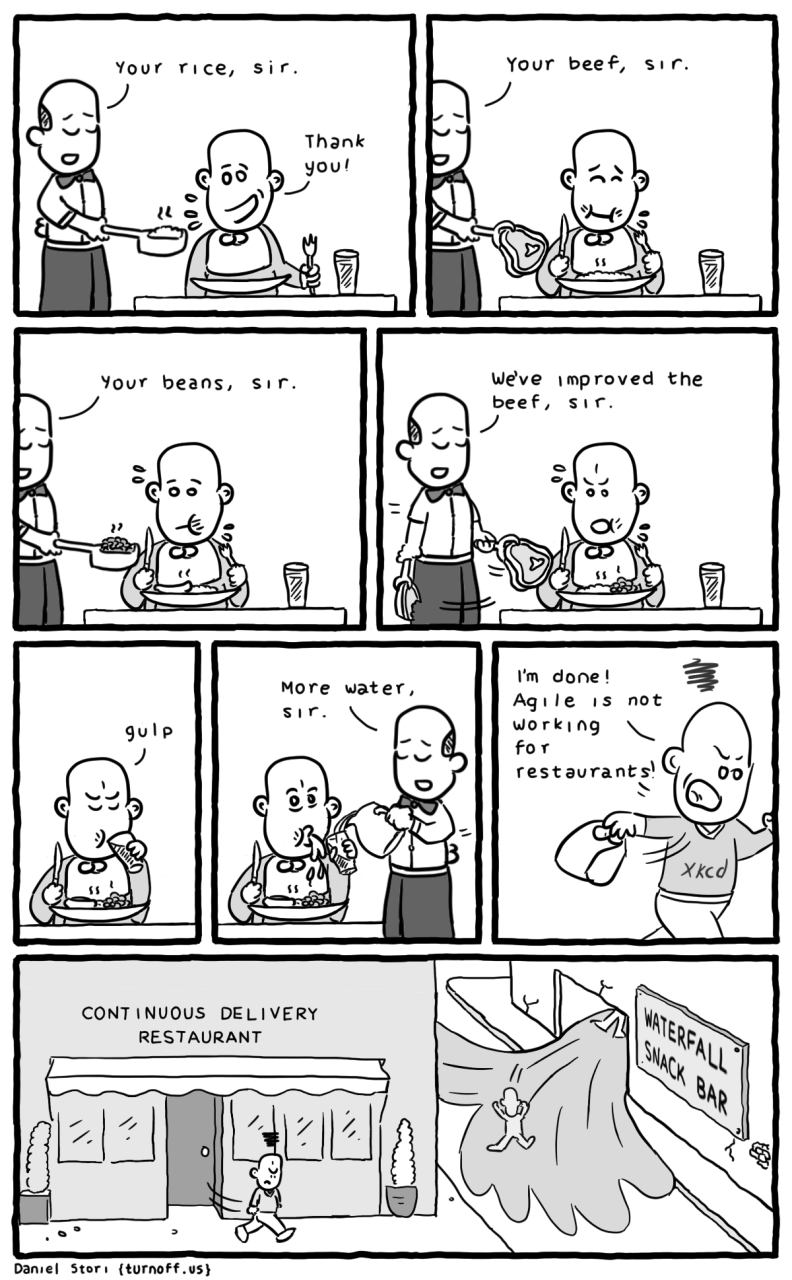
\includegraphics[width=0.9\textwidth]{fig/comic.jpg}
\end{center}
\caption{Usar metodologías ágiles no siempre es lo mejor}
\label{fig:comic}
\hrule
\end{figure}
